%% Jason Chalom 711985 Honours 2017

%% bare_jrnl.tex
%% V1.3
%% 2007/01/11
%% by Michael Shell
%% see http://www.michaelshell.org/
%% for current contact information.
%%
%% This is a skeleton file demonstrating the use of IEEEtran.cls
%% (requires IEEEtran.cls version 1.7 or later) with an IEEE journal paper.
%%
%% Support sites:
%% http://www.michaelshell.org/tex/ieeetran/
%% http://www.ctan.org/tex-archive/macros/latex/contrib/IEEEtran/
%% and
%% http://www.ieee.org/



% *** Authors should verify (and, if needed, correct) their LaTeX system  ***
% *** with the testflow diagnostic prior to trusting their LaTeX platform ***
% *** with production work. IEEE's font choices can trigger bugs that do  ***
% *** not appear when using other class files.                            ***
% The testflow support page is at:
% http://www.michaelshell.org/tex/testflow/


%%*************************************************************************
%% Legal Notice:
%% This code is offered as-is without any warranty either expressed or
%% implied; without even the implied warranty of MERCHANTABILITY or
%% FITNESS FOR A PARTICULAR PURPOSE! 
%% User assumes all risk.
%% In no event shall IEEE or any contributor to this code be liable for
%% any damages or losses, including, but not limited to, incidental,
%% consequential, or any other damages, resulting from the use or misuse
%% of any information contained here.
%%
%% All comments are the opinions of their respective authors and are not
%% necessarily endorsed by the IEEE.
%%
%% This work is distributed under the LaTeX Project Public License (LPPL)
%% ( http://www.latex-project.org/ ) version 1.3, and may be freely used,
%% distributed and modified. A copy of the LPPL, version 1.3, is included
%% in the base LaTeX documentation of all distributions of LaTeX released
%% 2003/12/01 or later.
%% Retain all contribution notices and credits.
%% ** Modified files should be clearly indicated as such, including  **
%% ** renaming them and changing author support contact information. **
%%
%% File list of work: IEEEtran.cls, IEEEtran_HOWTO.pdf, bare_adv.tex,
%%                    bare_conf.tex, bare_jrnl.tex, bare_jrnl_compsoc.tex
%%*************************************************************************

% Note that the a4paper option is mainly intended so that authors in
% countries using A4 can easily print to A4 and see how their papers will
% look in print - the typesetting of the document will not typically be
% affected with changes in paper size (but the bottom and side margins will).
% Use the testflow package mentioned above to verify correct handling of
% both paper sizes by the user's LaTeX system.
%
% Also note that the "draftcls" or "draftclsnofoot", not "draft", option
% should be used if it is desired that the figures are to be displayed in
% draft mode.
%
\documentclass[journal]{IEEEtran}
\usepackage{blindtext}
\usepackage[fleqn]{amsmath}
\usepackage{graphicx}
\usepackage[colorinlistoftodos]{todonotes}
\usepackage[colorlinks=true, allcolors=blue]{hyperref}
\usepackage{float}
\usepackage{algorithm}
\usepackage[noend]{algpseudocode}
\usepackage{listings}
\usepackage{enumerate}
\usepackage[final]{pdfpages}

\usepackage{color}

\definecolor{dkgreen}{rgb}{0,0.6,0}
\definecolor{gray}{rgb}{0.5,0.5,0.5}
\definecolor{mauve}{rgb}{0.58,0,0.82}
\definecolor{darkblue}{rgb}{0.0,0.0,0.6}
\definecolor{cyan}{rgb}{0.0,0.6,0.6}

 \lstset{frame=tb,
  language=C++,
  breaklines=true,
  showstringspaces=false,
  columns=flexible,
  numbers=none,
  commentstyle=\color{dkgreen},
  stringstyle=\color{mauve},
  tabsize=3
}
\lstdefinelanguage{XML}
{
  morestring=[b]",
  morestring=[s]{>}{<},
  morecomment=[s]{<?}{?>},
  stringstyle=\color{black},
  identifierstyle=\color{darkblue},
  keywordstyle=\color{cyan},
  morekeywords={xmlns,version,type,ma-id}% list your attributes here
}

\graphicspath{ {images/} }

\newenvironment{myitemize}
{ \begin{itemize}
    \setlength{\itemsep}{0pt}
    \setlength{\parskip}{0pt}
    \setlength{\parsep}{0pt}     }
  { \end{itemize}                  } 

\newcommand{\itab}[1]{\hspace{0em}\rlap{#1}}
\newcommand{\tab}[1]{\hspace{.2\textwidth}\rlap{#1}}
% \usepackage{enumitem}

% Some very useful LaTeX packages include:
% (uncomment the ones you want to load)


% *** MISC UTILITY PACKAGES ***
%
%\usepackage{ifpdf}
% Heiko Oberdiek's ifpdf.sty is very useful if you need conditional
% compilation based on whether the output is pdf or dvi.
% usage:
% \ifpdf
%   % pdf code
% \else
%   % dvi code
% \fi
% The latest version of ifpdf.sty can be obtained from:
% http://www.ctan.org/tex-archive/macros/latex/contrib/oberdiek/
% Also, note that IEEEtran.cls V1.7 and later provides a builtin
% \ifCLASSINFOpdf conditional that works the same way.
% When switching from latex to pdflatex and vice-versa, the compiler may
% have to be run twice to clear warning/error messages.






% *** CITATION PACKAGES ***
%
%\usepackage{cite}
% cite.sty was written by Donald Arseneau
% V1.6 and later of IEEEtran pre-defines the format of the cite.sty package
% \cite{} output to follow that of IEEE. Loading the cite package will
% result in citation numbers being automatically sorted and properly
% "compressed/ranged". e.g., [1], [9], [2], [7], [5], [6] without using
% cite.sty will become [1], [2], [5]--[7], [9] using cite.sty. cite.sty's
% \cite will automatically add leading space, if needed. Use cite.sty's
% noadjust option (cite.sty V3.8 and later) if you want to turn this off.
% cite.sty is already installed on most LaTeX systems. Be sure and use
% version 4.0 (2003-05-27) and later if using hyperref.sty. cite.sty does
% not currently provide for hyperlinked citations.
% The latest version can be obtained at:
% http://www.ctan.org/tex-archive/macros/latex/contrib/cite/
% The documentation is contained in the cite.sty file itself.






% *** GRAPHICS RELATED PACKAGES ***
%
\ifCLASSINFOpdf
  % \usepackage[pdftex]{graphicx}
  % declare the path(s) where your graphic files are
  % \graphicspath{{../pdf/}{../jpeg/}}
  % and their extensions so you won't have to specify these with
  % every instance of \includegraphics
  % \DeclareGraphicsExtensions{.pdf,.jpeg,.png}
\else
  % or other class option (dvipsone, dvipdf, if not using dvips). graphicx
  % will default to the driver specified in the system graphics.cfg if no
  % driver is specified.
  % \usepackage[dvips]{graphicx}
  % declare the path(s) where your graphic files are
  % \graphicspath{{../eps/}}
  % and their extensions so you won't have to specify these with
  % every instance of \includegraphics
  % \DeclareGraphicsExtensions{.eps}
\fi
% graphicx was written by David Carlisle and Sebastian Rahtz. It is
% required if you want graphics, photos, etc. graphicx.sty is already
% installed on most LaTeX systems. The latest version and documentation can
% be obtained at: 
% http://www.ctan.org/tex-archive/macros/latex/required/graphics/
% Another good source of documentation is "Using Imported Graphics in
% LaTeX2e" by Keith Reckdahl which can be found as epslatex.ps or
% epslatex.pdf at: http://www.ctan.org/tex-archive/info/
%
% latex, and pdflatex in dvi mode, support graphics in encapsulated
% postscript (.eps) format. pdflatex in pdf mode supports graphics
% in .pdf, .jpeg, .png and .mps (metapost) formats. Users should ensure
% that all non-photo figures use a vector format (.eps, .pdf, .mps) and
% not a bitmapped formats (.jpeg, .png). IEEE frowns on bitmapped formats
% which can result in "jaggedy"/blurry rendering of lines and letters as
% well as large increases in file sizes.
%
% You can find documentation about the pdfTeX application at:
% http://www.tug.org/applications/pdftex





% *** MATH PACKAGES ***
%
%\usepackage[cmex10]{amsmath}
% A popular package from the American Mathematical Society that provides
% many useful and powerful commands for dealing with mathematics. If using
% it, be sure to load this package with the cmex10 option to ensure that
% only type 1 fonts will utilized at all point sizes. Without this option,
% it is possible that some math symbols, particularly those within
% footnotes, will be rendered in bitmap form which will result in a
% document that can not be IEEE Xplore compliant!
%
% Also, note that the amsmath package sets \interdisplaylinepenalty to 10000
% thus preventing page breaks from occurring within multiline equations. Use:
%\interdisplaylinepenalty=2500
% after loading amsmath to restore such page breaks as IEEEtran.cls normally
% does. amsmath.sty is already installed on most LaTeX systems. The latest
% version and documentation can be obtained at:
% http://www.ctan.org/tex-archive/macros/latex/required/amslatex/math/





% *** SPECIALIZED LIST PACKAGES ***
%
%\usepackage{algorithmic}
% algorithmic.sty was written by Peter Williams and Rogerio Brito.
% This package provides an algorithmic environment fo describing algorithms.
% You can use the algorithmic environment in-text or within a figure
% environment to provide for a floating algorithm. Do NOT use the algorithm
% floating environment provided by algorithm.sty (by the same authors) or
% algorithm2e.sty (by Christophe Fiorio) as IEEE does not use dedicated
% algorithm float types and packages that provide these will not provide
% correct IEEE style captions. The latest version and documentation of
% algorithmic.sty can be obtained at:
% http://www.ctan.org/tex-archive/macros/latex/contrib/algorithms/
% There is also a support site at:
% http://algorithms.berlios.de/index.html
% Also of interest may be the (relatively newer and more customizable)
% algorithmicx.sty package by Szasz Janos:
% http://www.ctan.org/tex-archive/macros/latex/contrib/algorithmicx/




% *** ALIGNMENT PACKAGES ***
%
%\usepackage{array}
% Frank Mittelbach's and David Carlisle's array.sty patches and improves
% the standard LaTeX2e array and tabular environments to provide better
% appearance and additional user controls. As the default LaTeX2e table
% generation code is lacking to the point of almost being broken with
% respect to the quality of the end results, all users are strongly
% advised to use an enhanced (at the very least that provided by array.sty)
% set of table tools. array.sty is already installed on most systems. The
% latest version and documentation can be obtained at:
% http://www.ctan.org/tex-archive/macros/latex/required/tools/


%\usepackage{mdwmath}
%\usepackage{mdwtab}
% Also highly recommended is Mark Wooding's extremely powerful MDW tools,
% especially mdwmath.sty and mdwtab.sty which are used to format equations
% and tables, respectively. The MDWtools set is already installed on most
% LaTeX systems. The lastest version and documentation is available at:
% http://www.ctan.org/tex-archive/macros/latex/contrib/mdwtools/


% IEEEtran contains the IEEEeqnarray family of commands that can be used to
% generate multiline equations as well as matrices, tables, etc., of high
% quality.


%\usepackage{eqparbox}
% Also of notable interest is Scott Pakin's eqparbox package for creating
% (automatically sized) equal width boxes - aka "natural width parboxes".
% Available at:
% http://www.ctan.org/tex-archive/macros/latex/contrib/eqparbox/





% *** SUBFIGURE PACKAGES ***
%\usepackage[tight,footnotesize]{subfigure}
% subfigure.sty was written by Steven Douglas Cochran. This package makes it
% easy to put subfigures in your figures. e.g., "Figure 1a and 1b". For IEEE
% work, it is a good idea to load it with the tight package option to reduce
% the amount of white space around the subfigures. subfigure.sty is already
% installed on most LaTeX systems. The latest version and documentation can
% be obtained at:
% http://www.ctan.org/tex-archive/obsolete/macros/latex/contrib/subfigure/
% subfigure.sty has been superceeded by subfig.sty.



%\usepackage[caption=false]{caption}
%\usepackage[font=footnotesize]{subfig}
% subfig.sty, also written by Steven Douglas Cochran, is the modern
% replacement for subfigure.sty. However, subfig.sty requires and
% automatically loads Axel Sommerfeldt's caption.sty which will override
% IEEEtran.cls handling of captions and this will result in nonIEEE style
% figure/table captions. To prevent this problem, be sure and preload
% caption.sty with its "caption=false" package option. This is will preserve
% IEEEtran.cls handing of captions. Version 1.3 (2005/06/28) and later 
% (recommended due to many improvements over 1.2) of subfig.sty supports
% the caption=false option directly:
%\usepackage[caption=false,font=footnotesize]{subfig}
%
% The latest version and documentation can be obtained at:
% http://www.ctan.org/tex-archive/macros/latex/contrib/subfig/
% The latest version and documentation of caption.sty can be obtained at:
% http://www.ctan.org/tex-archive/macros/latex/contrib/caption/




% *** FLOAT PACKAGES ***
%
%\usepackage{fixltx2e}
% fixltx2e, the successor to the earlier fix2col.sty, was written by
% Frank Mittelbach and David Carlisle. This package corrects a few problems
% in the LaTeX2e kernel, the most notable of which is that in current
% LaTeX2e releases, the ordering of single and double column floats is not
% guaranteed to be preserved. Thus, an unpatched LaTeX2e can allow a
% single column figure to be placed prior to an earlier double column
% figure. The latest version and documentation can be found at:
% http://www.ctan.org/tex-archive/macros/latex/base/



%\usepackage{stfloats}
% stfloats.sty was written by Sigitas Tolusis. This package gives LaTeX2e
% the ability to do double column floats at the bottom of the page as well
% as the top. (e.g., "\begin{figure*}[!b]" is not normally possible in
% LaTeX2e). It also provides a command:
%\fnbelowfloat
% to enable the placement of footnotes below bottom floats (the standard
% LaTeX2e kernel puts them above bottom floats). This is an invasive package
% which rewrites many portions of the LaTeX2e float routines. It may not work
% with other packages that modify the LaTeX2e float routines. The latest
% version and documentation can be obtained at:
% http://www.ctan.org/tex-archive/macros/latex/contrib/sttools/
% Documentation is contained in the stfloats.sty comments as well as in the
% presfull.pdf file. Do not use the stfloats baselinefloat ability as IEEE
% does not allow \baselineskip to stretch. Authors submitting work to the
% IEEE should note that IEEE rarely uses double column equations and
% that authors should try to avoid such use. Do not be tempted to use the
% cuted.sty or midfloat.sty packages (also by Sigitas Tolusis) as IEEE does
% not format its papers in such ways.


%\ifCLASSOPTIONcaptionsoff
%  \usepackage[nomarkers]{endfloat}
% \let\MYoriglatexcaption\caption
% \renewcommand{\caption}[2][\relax]{\MYoriglatexcaption[#2]{#2}}
%\fi
% endfloat.sty was written by James Darrell McCauley and Jeff Goldberg.
% This package may be useful when used in conjunction with IEEEtran.cls'
% captionsoff option. Some IEEE journals/societies require that submissions
% have lists of figures/tables at the end of the paper and that
% figures/tables without any captions are placed on a page by themselves at
% the end of the document. If needed, the draftcls IEEEtran class option or
% \CLASSINPUTbaselinestretch interface can be used to increase the line
% spacing as well. Be sure and use the nomarkers option of endfloat to
% prevent endfloat from "marking" where the figures would have been placed
% in the text. The two hack lines of code above are a slight modification of
% that suggested by in the endfloat docs (section 8.3.1) to ensure that
% the full captions always appear in the list of figures/tables - even if
% the user used the short optional argument of \caption[]{}.
% IEEE papers do not typically make use of \caption[]'s optional argument,
% so this should not be an issue. A similar trick can be used to disable
% captions of packages such as subfig.sty that lack options to turn off
% the subcaptions:
% For subfig.sty:
% \let\MYorigsubfloat\subfloat
% \renewcommand{\subfloat}[2][\relax]{\MYorigsubfloat[]{#2}}
% For subfigure.sty:
% \let\MYorigsubfigure\subfigure
% \renewcommand{\subfigure}[2][\relax]{\MYorigsubfigure[]{#2}}
% However, the above trick will not work if both optional arguments of
% the \subfloat/subfig command are used. Furthermore, there needs to be a
% description of each subfigure *somewhere* and endfloat does not add
% subfigure captions to its list of figures. Thus, the best approach is to
% avoid the use of subfigure captions (many IEEE journals avoid them anyway)
% and instead reference/explain all the subfigures within the main caption.
% The latest version of endfloat.sty and its documentation can obtained at:
% http://www.ctan.org/tex-archive/macros/latex/contrib/endfloat/
%
% The IEEEtran \ifCLASSOPTIONcaptionsoff conditional can also be used
% later in the document, say, to conditionally put the References on a 
% page by themselves.





% *** PDF, URL AND HYPERLINK PACKAGES ***
%
%\usepackage{url}
% url.sty was written by Donald Arseneau. It provides better support for
% handling and breaking URLs. url.sty is already installed on most LaTeX
% systems. The latest version can be obtained at:
% http://www.ctan.org/tex-archive/macros/latex/contrib/misc/
% Read the url.sty source comments for usage information. Basically,
% \url{my_url_here}.





% *** Do not adjust lengths that control margins, column widths, etc. ***
% *** Do not use packages that alter fonts (such as pslatex).         ***
% There should be no need to do such things with IEEEtran.cls V1.6 and later.
% (Unless specifically asked to do so by the journal or conference you plan
% to submit to, of course. )


% correct bad hyphenation here
% \hyphenation{op-tical net-works semi-conduc-tor}


\begin{document}
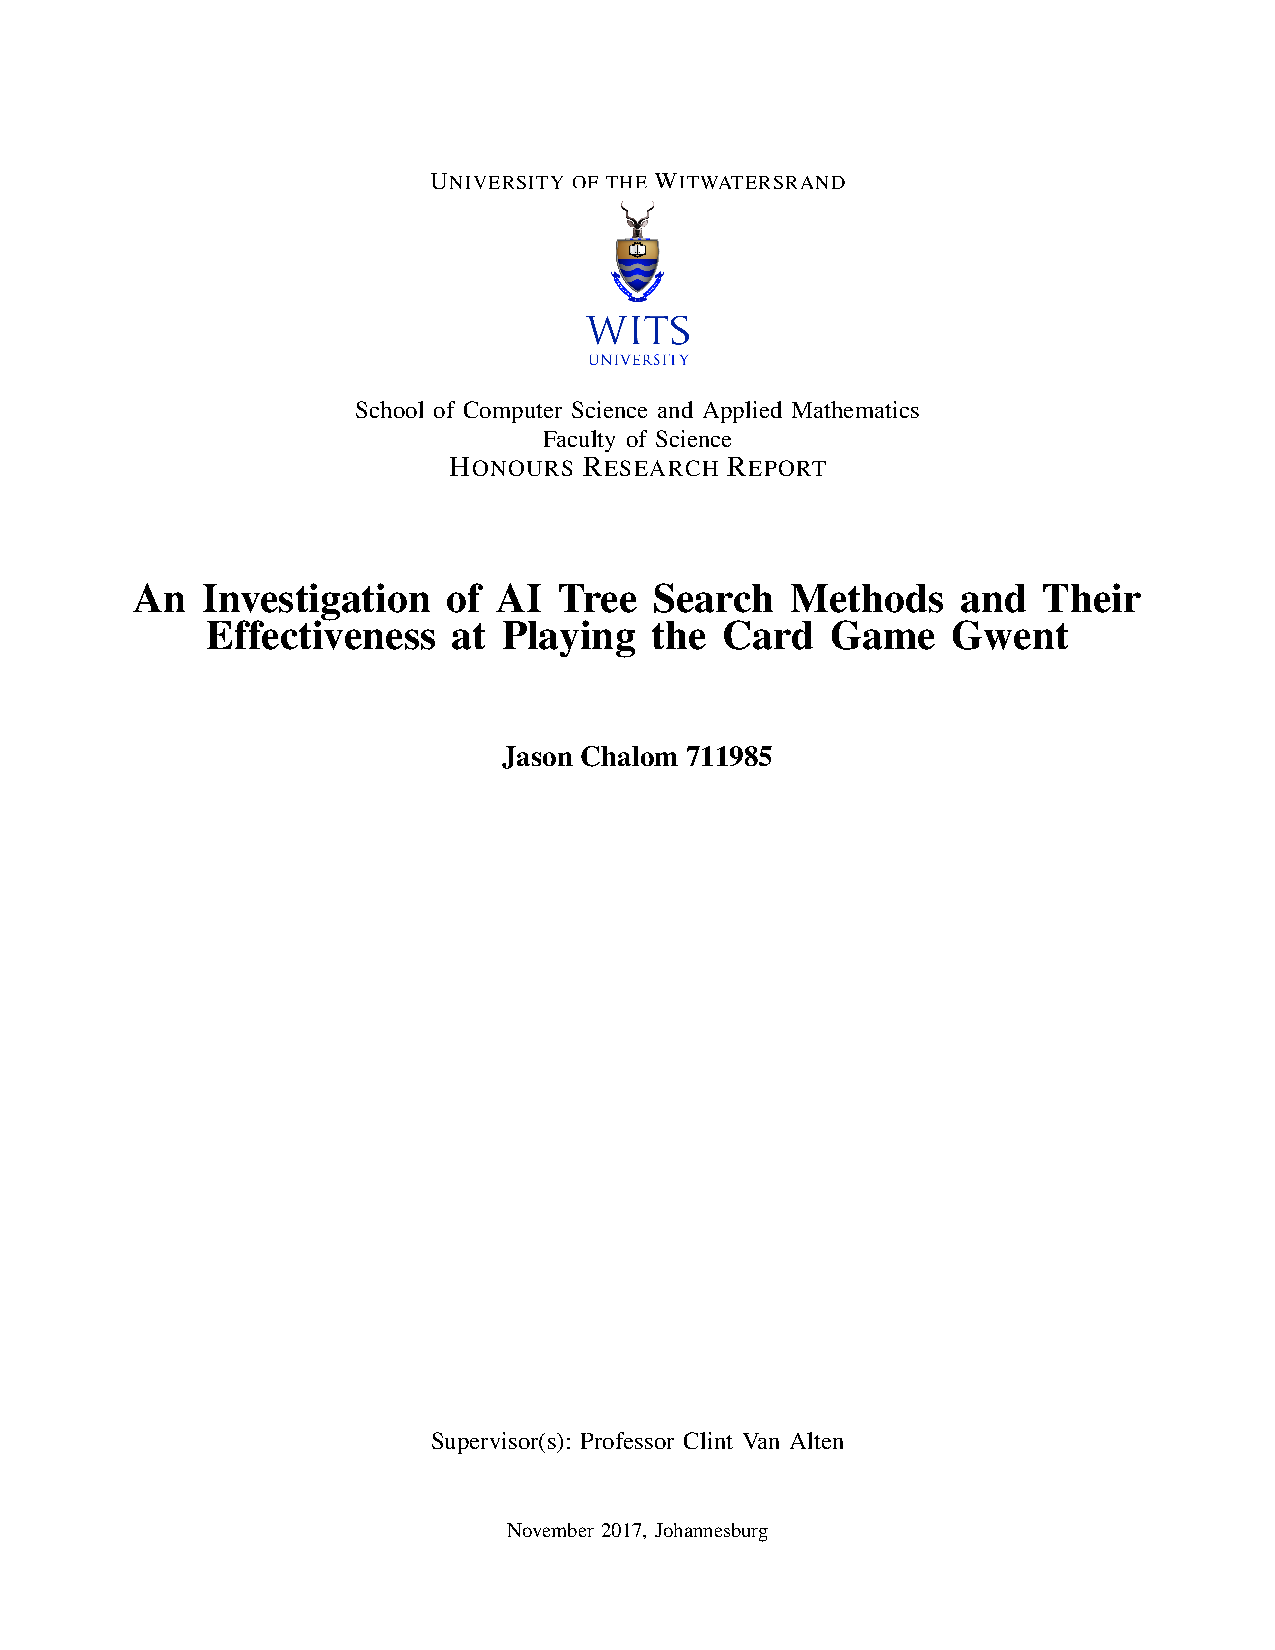
\includepdf[pages=-]{cover.pdf}
%
% paper title
% can use linebreaks \\ within to get better formatting as desired
\title{An Investigation of AI Tree Search Methods and Their Effectiveness at Playing the Card Game Gwent}
%
%
% author names and IEEE memberships
% note positions of commas and nonbreaking spaces ( ~ ) LaTeX will not break
% a structure at a ~ so this keeps an author's name from being broken across
% two lines.
% use \thanks{} to gain access to the first footnote area
% a separate \thanks must be used for each paragraph as LaTeX2e's \thanks
% was not built to handle multiple paragraphs
%

\author{Jason Chalom 711985}

% note the % following the last \IEEEmembership and also \thanks - 
% these prevent an unwanted space from occurring between the last author name
% and the end of the author line. i.e., if you had this:
% 
% \author{....lastname \thanks{...} \thanks{...} }
%                     ^------------^------------^----Do not want these spaces!
%
% a space would be appended to the last name and could cause every name on that
% line to be shifted left slightly. This is one of those "LaTeX things". For
% instance, "\textbf{A} \textbf{B}" will typeset as "A B" not "AB". To get
% "AB" then you have to do: "\textbf{A}\textbf{B}"
% \thanks is no different in this regard, so shield the last } of each \thanks
% that ends a line with a % and do not let a space in before the next \thanks.
% Spaces after \IEEEmembership other than the last one are OK (and needed) as
% you are supposed to have spaces between the names. For what it is worth,
% this is a minor point as most people would not even notice if the said evil
% space somehow managed to creep in.



% The paper headers
\markboth{University of the Witwatersrand, School of Computer Science and Applied Mathematics}%
{School of Computer Science and Applied Mathematics}
% The only time the second header will appear is for the odd numbered pages
% after the title page when using the twoside option.
% 
% *** Note that you probably will NOT want to include the author's ***
% *** name in the headers of peer review papers.                   ***
% You can use \ifCLASSOPTIONpeerreview for conditional compilation here if
% you desire.


% If you want to put a publisher's ID mark on the page you can do it like
% this:
%\IEEEpubid{0000--0000/00\$00.00~\copyright~2007 IEEE}
% Remember, if you use this you must call \IEEEpubidadjcol in the second
% column for its text to clear the IEEEpubid mark.


% use for special paper notices
%\IEEEspecialpapernotice{(Invited Paper)}


% make the title area
\maketitle


\begin{abstract}
%\boldmath
The aim of this research is to compare AI tree search methods when applied to the game Gwent. Gwent is an interesting domain because it is non-deterministic and has sub-domains which require their own search operations to be performed when decisions are made. Is Gwent random in nature or does the use of strategy affect the outcome of a game? Using empirical analysis on three random agents (and four more intelligent agents) it is shown that whilst Gwent has some random attributes the game itself is not random. Agents which are more geared towards strategic choices (such as MCTS) outperformed all other agents. It is also shown that the MCTS agent is the best agent for playing the game of Gwent but only when its parameter which controls the number of iterations is sufficiently large.

\end{abstract}
% IEEEtran.cls defaults to using nonbold math in the Abstract.
% This preserves the distinction between vectors and scalars. However,
% if the journal you are submitting to favors bold math in the abstract,
% then you can use LaTeX's standard command \boldmath at the very start
% of the abstract to achieve this. Many IEEE journals frown on math
% in the abstract anyway.

% Note that keywords are not normally used for peerreview papers.
% \begin{IEEEkeywords}
% Machine Learning, Artificial Intelligence, Gwent, MCTS, Tree Search, Pseudo-Random
% \end{IEEEkeywords}






% For peer review papers, you can put extra information on the cover
% page as needed:
% \ifCLASSOPTIONpeerreview
% \begin{center} \bfseries EDICS Category: 3-BBND \end{center}
% \fi
%
% For peerreview papers, this IEEEtran command inserts a page break and
% creates the second title. It will be ignored for other modes.
\IEEEpeerreviewmaketitle



\section{Introduction}
  The textbook, Artificial Intelligence: A Modern Approach \cite{AIModern} describes games as having been an area of interest for humans since the beginning of organised societies. A game is where two players or agents are in competition in some domain with a defined set of rules. Research in artificial intelligence (AI) has always gravitated towards games due to the complexity and abstractedness they present and yet they have clearly defined rules which make them easier to program and study than other abstract real-world problems such as physical sport. The applications of AI in games can lead to developments in other more serious fields such as applications in economics. \\
  
  Not all games are the same. Artificial Intelligence: A Modern Approach \cite{AIModern} describes many games such as deterministic games where the outcomes are known, turn based games where each player must wait their turn, two-player games and zero-sum games where in a multi-player arena only one player can win as whatever gains (wins) one player gets the other player must then lose out on. A game with perfect information means that both players know full-well what the outcomes of all previous moves were. \\
  
  Games are an interesting area of study because of how difficult they can be. Many games are computationally difficult to solve - both in complexity and time. Some games can have so many states that would have to be computed that it is in-feasible to calculate all of them within the time constraints of a game where inefficiency could have penalties. Also due to the very nature of deriving game decisions and paths for future moves, having branching factors which depend on the types of games being solved will produce exceedingly large solution spaces. This means that strategies which employ smart use of resource constraints in a given domain are required to solve these problems. \cite{AIModern}. 
  
  \subsection{Problem Domain: The Card Game Gwent}
  The Gwent game guide \cite{guide} describes Gwent as a two-player turn-based card game based on a medieval (fantasy) battle field. It is a game played to the best of three rounds where the players use the same hand of cards drawn from their respective shuffled decks prior to start of play. Each player creates a deck from the total cards they have based on a certain faction and they choose cards whilst following a set of rules which govern how theses decks should be constructed. There are a few different rule sets and as new cards are introduced to the game new rules may be added. This game is interesting because it is a zero-sum game with partial information. The players both know the moves which came before but they do not know the opposing players hand. Gwent has a number of interesting rules such as there being a card which allows a player to select a card from their discard pile and playing it again. Another interesting card is one which the player plays on the opposing side of the board. Here the card acts against the player who played the card in return for two new cards from the player’s deck.

  \begin{figure}[H]
    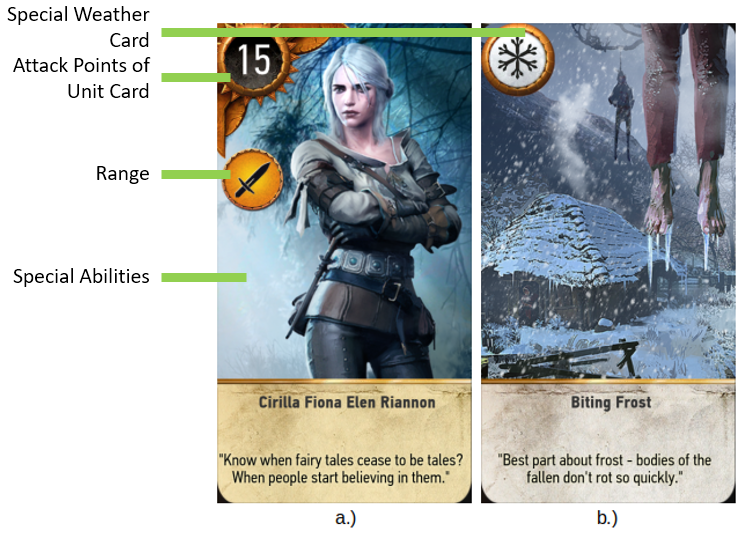
\includegraphics[width=.45\textwidth,scale=.45]{card}\\
    \centering
    \caption{Example of a unit Gwent Card (a) and a weather/special card (b). \cite{guide} \cite{cdp}}
  \end{figure}
  
  \subsection{Aim of Research}
  Gwent is an unknown domain in terms of how different variants of tree search algorithms such as MCTS may perform. A search through existing literature has not found any research which applies these methods to this exact problem. Gwent is also a relatively new game which is still being actively developed \cite{cdp} which may explain the lack of its use in existing literature. I wanted to prove that the game of Gwent is not a purely random game of chance but rather that a well implemented strategy will determine the outcomes of a game. If this is true then random agents should perform poorly when compared to more advanced AI agents.\\

  \subsubsection{Hypothesis}
  My hypothesis states that:\\
  \indent\textbf{The game of Gwent is not random in nature and therefore AI agents will have higher win rates when compared to random agents.}
  
  \section{Background and Related Research}
  \label{background}

  \subsection{The Rules of Gwent}
  Gwent is a 2-player turn-based game, with three rounds \cite{guide}. The game is the best of three rounds. Each player must have a chosen deck which consists one leader card, twenty-two unit cards minimum, and ten special cards maximum. Unit cards which are hero cards, cannot be revived or effected by any other card. Ten random cards from the chosen deck are drawn at the start of the three rounds for both players. Each player takes a turn placing one card on the board. The board has three rows on both sides. Certain units can only be placed on certain rows. A player can also at any turn decide to pass the remainder of the round. The winner of a round is decided when either both players run out of cards, both players pass the round or a combination of the two. A round win is calculated by adding up the strength of all unit cards whilst taking into account the effects of the special cards.
  \\\\\\
  \noindent \textbf{Special Cards:}
  
  \begin{itemize}
    \item There are four types of weather cards, one clear and one for each row of the battlefield (on both sides). The weather cards reduce all unit cards except hero cards to attack points equal to one (unless commanders horn is in effect then attack points of two).
    \item The commander's horn doubles attack points of all normal unit cards in that row.
    \item Scorch destroys the strongest valued cards on the board (i.e. the highest number, any card with that number is discarded)
    \item Decoy allows a player to take a card back into their hand.
  \end{itemize}
  
  \noindent \textbf{Abilities of Some Unit Cards}:
  \begin{itemize}
    \item Spy units go to the other player’s side in return for drawing two new cards from the player's deck into their hand.
    \item Medic allows you to look through the player's discard pile and revive one unit card (must not be a special or hero card).
    \item Tight bond doubles the attack points of a group of cards of the same type of unit (with this ability) when they are placed next to one another (The doubling is calculated on the combined strength of every card in the group).
  \end{itemize}
  
  \subsection{Literature Review}
  \subsubsection{AI Tree Searches}
  The basic idea of using tree searches to make decisions in game problems is to model the problem (or domain) as a set of decisions which are in the form of a tree. Each node of the tree as described by Artificial Intelligence: A Modern Approach \cite{AIModern} are specific game states and each edge of the tree is a certain decision or a certain path which can be taken from the parent node to get to the children nodes or the next set of possible game states. The root of the tree is either the current state of the game or the initial state depending on the implementation of tree search. A terminal node on a tree is a node where either the game has reached a stop (or end) state such that no further children can be created or a limiting condition has been met which limits the depth of the tree.\\
  
  \subsubsection{Tree Pruning}
  One notable problem with the approach of generating trees based on possible domain states of a game is the sheer size and complexity which can emerge from many games such as Gwent and its contemporaries. Edwards et al. \cite{AIM030} and in chapter 5 of Artificial Intelligence: A Modern Approach \cite{AIModern} both describe how a tree constructed from all possible game states is wasteful as there are many branches which need not be considered. The growth of these trees are exponential in nature (based on the size of the domain being modelled and searched) which creates a problem of time and complexity when dealing with the implementation of such an AI. In such cases these paths can be removed from the tree because they have no effect on the outcome of the tree search. This can greatly reduce the size of the tree before a complete search is done. \\
  
  Another approach as described by Chaslot et al. \cite{progressive} is to only invalidate a node (and therefore the rest of the path that follows) which is determined to be unreliable (or as a node not visited often in a tree search) and then these nodes can be re-evaluated and selected later (based on the search algorithm utilised).\\
  
  \subsubsection{Minimax Algorithm}
  Having created a tree of possible paths and game states an algorithm is needed to help determine which is the most optimal path for the AI to take in order to maximize its chances of winning the game (thereby minimize the chances of the other player from winning). This sets up the AI player as the MAX player and the opponent as the MIN player. One of these algorithms is called The Minimax Algorithm. Artificial Intelligence: A Modern Approach \cite{AIModern} describes this algorithm as a method of finding an optimal set of strategies. This is done by placing a value on each node of the tree which is called the Minimax value. This value is a numerical representation of how useful that decision is for the MAX Player i.e. the MAX player favours a higher value and the MIN player favours a lower value. In this set-up, for each decision that MAX makes, MIN must also make a decision and these two decisions together make-up one move on the tree - this is the basis of a multi-player game. These "half-moves" are defined by Artificial Intelligence: A Modern Approach \cite{AIModern} as a ply. The Minimax decision is the decision which leads to the optimal outcome for MAX from the root node. This algorithm will recursively generate the Minimax values for every child node in the tree by using an objective function which determines the numerical outcome of that specific node. Then the algorithm back-propagates up the tree updating the Minimax value of the parent nodes until root is reached where it terminates. \\
  \\
  \begin{figure}[H]
    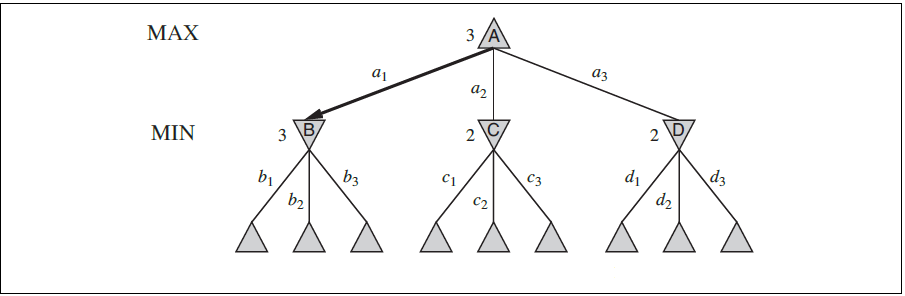
\includegraphics[width=.50\textwidth,scale=.50]{minimax}\\
    \centering
    \caption{Example of a Max tree where the Max nodes are the upright triangles and the Min nodes are down facing triangles, taken from Chapter 5 of Artificial Intelligence: A Modern Approach \cite{AIModern}.}
    \label{ab}
  \end{figure}
  
  One note which is made by Artificial Intelligence: A Modern Approach \cite{AIModern} on this algorithm is that there is an inherent assumption that both MAX and MIN play optimally. Also the Minimax algorithm in its most basic form will perform a full depth-first search of the tree which means that it will have an exponential growth in time complexity which corresponds to the exponential growth of the tree based on the domain space. The space complexity of this algorithm and the time complexity are determined by the depth of the tree and number of moves at each layer of the tree.\\
  
  \subsubsection{Alpha-Beta Pruning}
  The Alpha-Beta Pruning Heuristic was conceived as an extension of the Minimax algorithm. Edwards et al. \cite{AIM030} states that it uses partial information from the tree to decide which branches on the tree are no longer needed for Minimax. These removed branches do not affect the final decision determined by Minimax. The method uses the fact that if a move is found to be worse than a move evaluated previously (either for the MIN player or the MAX player), than that move does not affect the outcome of the search. Edwards et al. \cite{AIM030} highlights the importance of the ordering of the possible set of plies from the current node (position) because this heuristic achieves the best results when the optimal decision is located at the beginning of the set of positions. To this effect the Alpha-Beta Heuristic can at most cut a search trees growth rate in half, which implies that this heuristic allows a computing system to search twice the depth within the same time complexity of the basic Minimax algorithm. Edwards et al. \cite{AIM030} proves this by induction in their technical memo. This performance increase is a powerful first step in using Minimax in a real world domain.
  \\
  \begin{figure}[H]
    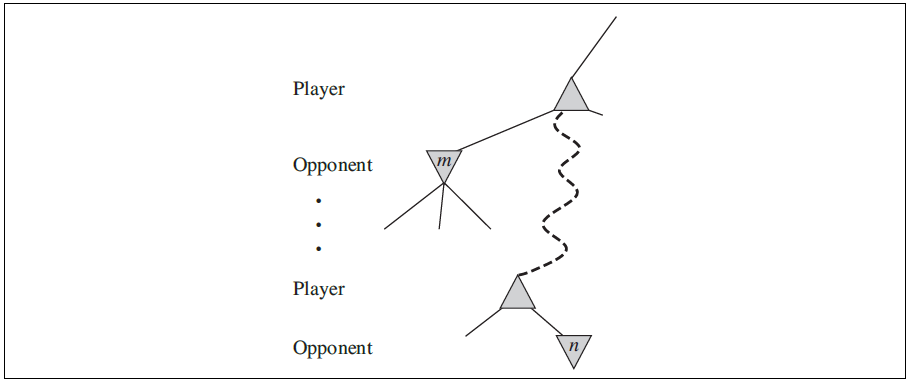
\includegraphics[width=.50\textwidth,scale=.50]{ab}\\
    \centering
    \caption{General case of alpha-beta pruning where if m is a better move than n, n will be removed, taken from Chapter 5 of Artificial Intelligence: A Modern Approach \cite{AIModern}.}
    \label{ab}
  \end{figure}
  
  % \subsubsection{Other Modifications to Minimax}
  % Chapter 5 of Artificial Intelligence: A Modern Approach \cite{AIModern} provides several other heuristics that can be applied to Minimax in order to deal with the exponential growth issue. These include having a cut-off condition which will only generate a tree up to a certain depth in order to contain the tree for use with computing systems which have inherent limitations. The games themselves may have limitations such as the amount of time available for making a decision. Another strategy which may be able to improve the effectiveness of Minimax in domains which are stochastic in nature and may only have partially observable information is by using Monte-Carlo simulations to generate probable states where the information is not certain. A third idea that was presented is to create a look-up table and store a set of known polices (or game heuristics) such as end states and killer moves which have proven to be effective in the past (or come from expert knowledge) and then use the look-up table when needed to make these specific decisions instead of running through a lengthy search. Such searches may then use approximations of moves past a certain depth in the tree as described by Chaslot et al. \cite{progressive} to determine most moves but retain the optimal pre-computed moves which such approximations may not choose due to the introduced error of the approximation.\\
  
  \subsubsection{Monte-Carlo Tree Search Algorithm}
  The basic idea of MCTS as described by James et al. \cite{wits} and Browne et al. \cite{survey} is that it combines the idea of a tree search with the idea of simulating parts of the domain space. Monte Carlo simulations are used to make approximations of some problem based on random sampling of the problem domain \cite{survey}. Browne et al. \cite{survey} describes MCTS as a family of heuristic optimisation methods for making optimal decisions in certain domains and game spaces. The basic operation of these methods sample the domain space (in similar fashion to MC methods) by simulation which is then used to build a search tree based on this sample of the domain. These methods work well with difficult problems such as hidden domains and problems where other techniques have been unsuccessful since they are stochastic in nature.\\
  
  Browne et al. \cite{survey}, James et al. \cite{wits} and Chaslot et al. \cite{progressive} all describe a basic construction of a MCTS as having four major steps: Selection, Expansion, Simulation (also known as roll-outs \cite{wits}) and Back-propagation The selection step is when the tree is traversed from the root node through to the most urgent terminating nodes of the tree - which is decided by some predefined policy. Chaslot et al. \cite{progressive} describes four ways of determining the best child node as the final move selection. These look at how often a child is visited, the value of the respective child and some combination of these and other parameters. The expansion step is when one or more children are added to the selected terminating node. A simulation is then run on the new expanded nodes to determine what the outcome of those actions could be in the future. The simulations are also governed by a policy, which in the most basic case is to perform a random move. Finally this result is back-propagated up the selected path to update the outcomes of this path (up to the root node). This process is repeated until a termination condition is met such as a limit on the number of iterations, or the size complexity of the search tree.
  \\
  \begin{figure}[H]
    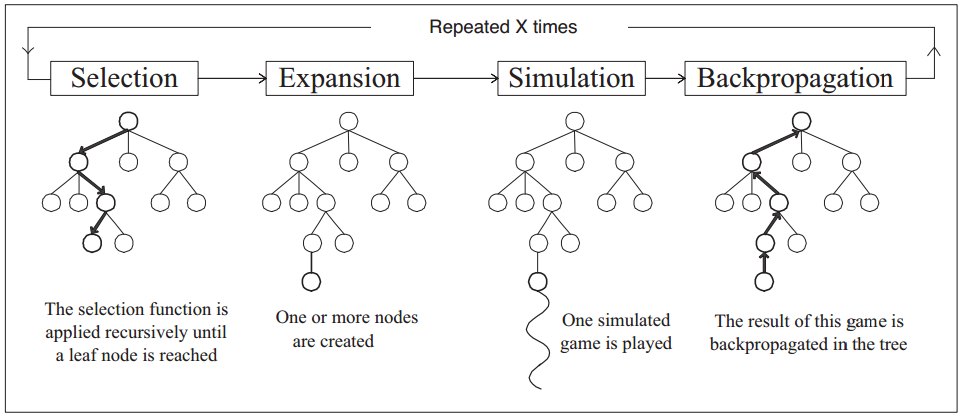
\includegraphics[width=.50\textwidth,scale=.50]{mcts}\\
    \centering
    \caption{Steps of the Monte-Carlo Tree Search, taken from Chaslot et al. \cite{MCTS_begin}.}
    \label{mcts}
  \end{figure}
  
  \subsubsection{The Use of Expanded Techniques with MCTS}
  Browne et al. \cite{survey} describes many different optimizations and enhancements to the basic MCTS and shows that there are many variants of MCTS which change different aspects of the four components of the algorithm.
  \\\\
  \textbf{Upper Confidence Bounds for Trees}\\\\
  Bandit based methods as used with MCTS are a modification of the selection phase of MCTS \cite{survey}. Browne et al. \cite{survey} describes bandit-based problems as a set of problems where there is an exploration-exploitation dilemma. This dilemma is that there is contention between the explorations of deeper variant moves with high win rate versus moves with few simulations associated with them (for the case of MCTS). Kocsis et al. \cite{bandit} applied a specific bandit algorithm for MCTS, known as UCB1. This application of a bandit-based policy for MCTS is known as the UCT algorithm. Here the algorithm uses random probabilities based on a policy mapping of what the next move that will be decided (as is generated in the expansion step). These generated moves are then checked against a regret (objective) function with the aim of minimizing the regret. The regret function used calculates the loss based on how many times the policies did not use the best possible path. The UCT algorithm, treats every child node of the move selection which has been explored as separate multi-armed bandit problems. The arms of each bandit problem are the available moves on the sub-tree and the child nodes are the weighted rewards of the paths calculated using the bandit-algorithm. During testing Kocsis et al. \cite{bandit} found that UCT appeared to produce a lower error than AB, MCTS and Monte-Carlo planning with Minimax value update (A hybrid approach to tree search).\\
  
  James et al. \cite{wits} have however discovered that UCT operates far better when there is a preservation of the optimal decision rankings. This is very similar to what Edwards et al. \cite{AIM030} found with AB pruning. Caution must then be taken when using the UCT method as James et al. \cite{wits} found that if the distributions of the random simulations have small variances than UCT can become sub-optimal and even worse than random. James et al. \cite{wits} noted that there has been a vast amount of work in researching alterations (such as UCT) in the selection and expansions steps of MCTS but less work has been done in the simulation step. 
  \\\\
  \textbf{Progressive Strategies for MCTS}\\\\
  Chaslot et al. \cite{progressive} suggested two progressive strategies which leave out infrequently visited nodes that can be selected and examined later. This is done using available information and some heuristics (which are computationally expensive) to select nodes which are visited often and invalidate the rest.\\
  
  Progressive bias as presented by Chaslot et al. \cite{progressive} and described in depth by Browne et al. \cite{survey} is a method which attempts to replace unreliable nodes (not visited often) with some heuristic function which takes in this suspect node as its input. This method works on the selection and expansion steps of MCTS. As the node is visited more (as the number of iterations of MCTS increases), the method will ensure that the heuristic's influence decreases. The heuristic may also only be applied after some fixed number of visits have passed for each node under question. This means that initially the MCTS functions as normal, after sometime the selection algorithm is applied to each node so the children with the highest heuristic values get chosen first due to there not being enough simulations to make an accurate prediction. As the number of simulations grows, the impact of both the heuristic function and the simulations are balanced. As the number of simulations keeps growing a boundary will be reached (determined by
  the heuristic function used) where the influence of the heuristic function will decrease until it has little effect whereas the effects of the simulated results now have a high impact on the outcome and the behaviour becomes similar to the basic approach of MCTS. \\
  
  Progressive unpruning is another method detailed by Chaslot et al. \cite{progressive} and described by Browne et al. \cite{survey} as a soft pruning method where possible decisions are ignored but may be evaluated later by using heuristic knowledge to reduce the size of the tree. This algorithm works when the number of simulations of some node equals a predefined threshold, a heuristic is then used to invalidate the less likely to be visited children nodes such that only the most likely nodes are selected. As the number of simulations gets bigger and further from the threshold, the children nodes should be progressively unpruned so that they may be evaluated. This reduces the number of sub-branches to deal with during the lower set of iterations of MCTS. Chaslot et al. \cite{progressive} has shown that this method helps with the time-complexity of the MCTS whilst improving the accuracy for a lower number of samples (simulations) when using MCTS. This provides the benefit that better results with lower error can be produced in a smaller time complexity than the vanilla MCTS.\\\\
  
  \textbf{Using Biasing Techniques with MCTS (Expert Knowledge)}\\\\
  Whitehouse et al. \cite{knowledge} proposed a method for initially biasing MCTS so that their commercial AI would seem more human to human players of their game. Their algorithm ISMCTS guesses potential game states and generates a game tree from the statistics of many potential game states by running simulations. Each iteration of the algorithm generates a new tree. They found that the injection of heuristic knowledge in MCTS was easier to implement than an expert heuristic system. They limited ISMCTS to only make decisions which can be contained in one round of their game because this algorithm is unable to look ahead to future rounds. The approach taken was to bias the initial selection step of MCTS and as the algorithm runs the applied bias tends to zero thereby avoiding the issue of weakening the AIs ability to take the best move for that round. The bias values are derived from existing knowledge. The tendency of the bias to go to zero is enforced during the back-propagation step when the updates of the node values which have a bias greater than 1 get their rewards increased whereas bias values less than 1 get reduced rewards. Whitehouse et al. \cite{knowledge} found that the MCTS chose the wrong move less than five percent from the tests conducted which was expected due to the random nature of the algorithm.\\
  
  There is however contention between Whitehouse et al. \cite{knowledge} and James et al. \cite{wits} as the former expects the injection of expert knowledge (bias) into MCTS will decrease the accuracy of the algorithm in choosing the most optimal decision whereas James et al. \cite{wits} found that the choice of bias is important in making sure that the performance of MCTS is not negatively affected and in some cases MCTS can perform better with bias added to the algorithm. There are some game problems where there is so little information supplied that running enough simulations to overcome this gap is in-feasible - a solution here would be to use an informed simulation. \\
  
  \subsubsection{The Idea of Hybrid Tree Searches}
  Baier et al. \cite{hybrids} highlights that Minimax search techniques are very good at selecting the most optimal strategies but at the cost of performance whereas MCTS is very good at dealing with large and complex search domains (such as incomplete information) but at the cost of error - in some cases missing critical decisions which Minimax would not miss. Baier et al. \cite{hybrids} puts forward different areas of MCTS which can be modified to use the Minimax search. The MCTS used in their experiments is the UCT form of the algorithm. A method which Baier et al. \cite{hybrids} described in the literature is to merge MCTS and Minimax is to use shallow (1-ply or 2-ply) searches at every simulation executed in MCTS - this however assumes the existence of an objective function and that the problem does not have incomplete knowledge.\\
  
  % Baier et al. \cite{hybrids} goes on to describe three different approaches to merging MCTS and Minimax search, one in the simulation step of MCTS, another across the selection and expansion steps and a third in the backpropagation step of MCTS.
  % \\\\
  % \textbf{Minimax in the Simulation Step (MCTS-MR)}\\\\
  % Rather than using uniformly random polices in the simulation step of MCTS rather Baier et al. \cite{hybrids} suggests Minimax searches of limited depth should be used to determine simulated decisions. However their method does not allow for objective functions so if Minimax cannot find a win or a loss than a random move must still be used. The power of this strategy is that certain errors which can occur when a random move is selected can be mitigated.
  % \\\\
  % \textbf{Minimax in the Selection and Expansion Steps (MCTS-MS)}\\\\
  % Here Baier et al. \cite{hybrids} experimented in using Minimax searches at any node in the selection and expansions steps of MCTS which are determined by a given heuristic. Two heuristics suggested are to use a condition which checks the number of times a node has been visited, or use a threshold based on the loss of a certain path or a heuristic condition which will initiate a Minimax search if a simulation is found to be quick. A quick simulation suggests there is a terminal node close to the current node. This strategy can help with keeping unnecessary paths off the search tree whilst keeping nodes of importance (win-paths) in the tree.
  % \\\\
  % \textbf{Minimax in the Backpropagation Step (MCTS-MB)}\\\\
  % Baier et al. \cite{hybrids} uses Minimax whenever the backpropagation step of MCTS has to switch from proven win/loss simulated returns to regular win/loss returns. This is caused when there are win states in child nodes whose parents are marked as a loss decision. Minimax is able to consider both terminal nodes and previous nodes (from previous MCTS iterations) which allows the algorithm to tell for which paths the opponent has a proven win. This strategy helps in making decisions be excluded more efficiently. A similar trick to MCTS-MS is to not use Minimax on sub-regions of the search domain where there are few terminal nodes (in the search tree).\\
  
  % Baier et al. \cite{hybrids} found that MCTS-MS and MCTS-MB have a significant improvement in performance over the vanilla MCTS whereas MCTS-MR is not as flexible in terms of different search domains as the other two algorithms. \\
  
  \textbf{Beam Monte-Carlo Tree Search}\\\\
  Baier et al. \cite{BEAM} describes BMCTS as a hybrid tree search where MCTS is combined with a beam search down the decision paths. A beam search is a search where more promising nodes are expanded whilst other nodes get rejected. This is done to reduce the memory and search complexities of a problem. It this hybrid approach the beam search acts as a pruning device for the MCTS tree. The pruning takes place during the back-propagation phase. The condition of pruning used in this approach is the number of simulations that have run through a node. The algorithm will keep the most visited node, remove the least visited nodes and the nodes at depth \emph{d} will no longer be created. Nodes beyond depth d will still continue to be explored. Only the retained nodes are taken into account which means that a sub-optimal solution may be found but the size of the potential tree is drastically reduced.\\

  \subsubsection{Testing Methodologies}
  \label{testing}
  James et al. \cite{wits} defined domains specifically for their testing purposes. They used grid world and finite MDPs to produce less complex problems in which to conduct their experiments. They then ran the different algorithms and a basic random agent over these domains to get their results which they then took averages of by running thousands of the same experiment sets.  Whitehouse et al. \cite{knowledge} had a set domain in which they had to work with. Here testing was done using AI-versus-AI simulations and using a select number of real people to beta test different versions of their AI. Chaslot et al. \cite{progressive}, Browne et al. \cite{survey} and Kocsis et al. \cite{bandit} used many domains (2 or more) to run their experiments and to also see if the domain space itself could cause these different methods to behave differently.\\
  
  \section{Research Methodology}
  \subsection{Introduction}
  The proposed methodology attempts to uses similar strategies as seen in the literature under Testing Methodologies (section \ref{testing}). An example is using AI-versus-AI simulations to find which AIs perform better than other AIs.
  
  \subsection{Restrictions Placed on the Domain}
  A sub domain of Gwent must be chosen in order to limit the scope of this research so that it will be feasible in the allotted time-frame. The chosen decks were limited to two decks which have cards already chosen so that the decks have similar attributes. The AI only decides on choices in the current hand and does not construct any decks prior to the game. These decks keep some of the special rules of the game such as being able to revive discarded cards but will not contain cards which can target specific opponent cards. The leader cards and their abilities will also be ignored. All AI (player) responses are limited by an iteration limit as this ensured that the many experimental games that need to be run could be done in a realistic time-frame.
  
  \subsection{Experimental Method}
  A game supervisor was built which produces the domain and enforces the rules of the game. The AIs also use it as a framework for their simulations and interactions with the game. Several AIs using versions of MCTS were made. A unit testing framework was also utilised in order to check that the implemented rules work as expected. Random AI agents who play random moves from a valid move list (for that game state) were also produced. 
  All the AIs must be run against the random agents to determine if they perform better than random on the domain. A tournament setting will then be setup where different AIs will be pitted against each other in a round-robin style to find which algorithms perform the best. This will be done in rounds of experiments where AI opponents will be set so that a large enough set of results can be collected and analysed to determine which AIs are better for each group of experimental rounds. Each individual experiment in a round will pit the same two AIs but the game state that is set will be randomly generated based on the available cards. Each experiment is run twice with the players swapped (which means swapping the decks as they are associated with players) - this is done to ensure fairness of the matches. Three pseudo-random agents are used to see what effect the PRNG has on the results.  
  
  \subsection{Implementation}
  The programming for the game supervisor and all the AI methods was done in C++. As described by Bronson et al. \cite{bronson2012c++} C++ allows for the use of inheritance techniques which allows for concepts such as the base tree implementations to be shared between the different AI implementations. C++ is also a compiled language which provides lower level access to a computer systems resources which allowed me to make code which runs faster than equivalent code in an interpreted language's virtual environment. Another useful implication of using C++ is that many advanced parallel computing libraries such as OpenMP are extensions of C and C++ \cite{parallel}. Many parts of the testing system has been parallelised in order to speed up independent parts of the simulation such as random roll-outs which are mutually exclusive of each other. All the AI implementations make use of game supervisor classes.\\

  \subsubsection{Random Agents}
  I used Marsaglia's xorshift generator \cite{marsaglia} \cite{XOR}, the well known Fast-Rand PRNG \cite{frand} and the Mersenne Twister 19937 generator (which is a built into c++11, and recommended to be used) as the PRNGs for my random agents \cite{mt}. These PRNGs are used to generate a random number which is in the range of the number of cards in that player's (agent's) hand. The agent then returns the corresponding card to be played by the framework.\\

  \subsubsection{Heuristic Agent}
  The heuristic player uses the equation \ref{eq:1} where the reward is between $-1$ and $1$. This Heuristic takes into consideration the current attack-points each player has in play for that round, the number of cards left in each player's hands and the number of round wins - which is weighted more heavily. The reason the terms are normalized is so that their influence with regards to the reward is weighted according to the observed importance of each term within the game.

  \begin{equation} \label{eq:1}
  \begin{split}
  \begin{aligned}
    reward =  0.2 \text{ X } \text{(AttackPoints - EnemyAttackPoints)}  &+\\
              0.2 \text{ X (HandSize - EnemyHandSize)}  &+\\
              0.6 \text{ X (RoundWins - EnemyRoundWins)}  &
  \end{aligned}
  \end{split}
  \end{equation}
  \\
  \subsubsection{Random Roll-out Agent}
  The random roll-out agent iterates through its own hand (deck). For each card it simulates an entire random game (to the end of the game) and will repeat the simulations based on the limit defined by the variable numberOfIterations. This limit is set to $1000$ iterations for most of the experimental runs. For each simulation it records the wins, draws and losses and when the agent finishes it will return the move (Card) with the most wins. This agent uses OpenMP to parallelise the simulations run for a given card. \\

  \subsubsection{MCTS Agent}
  This agent follows the MCTS framework as defined by Baier et al. \cite{BEAM}. The selection phase will initially select randomly (using the Mersenne Twister approach) and as the tree begins to develop it will select based on the back-propagated UCT values for each node (in the tree). This phase uses the default UCB1 sampling algorithm. The cumulative reward which is used during the back-propagation phase is a decimal number between $-1$ and $1$. If there is a win for the agent for a specific roll-out then $1.0$ is added to the specific node being computed. If there is a draw than $0.5$ is awarded, otherwise if there is a loss than $-1$ is added to that node. The back-propagation step calculates the value of each node by dividing the cumulative reward at that node by the number of times the node has been visited. This agent also has a limiting parameter numberOfIterations which is set to $1000$ iterations for most of the experimental runs.
  \\
  \subsubsection{MCTS2 Agent}
  This agent modified the basic MCTS framework so that pruning of the tree takes place at every iteration of the algorithm. Rather than using the BMCTS algorithm to prune the tree based on a heuristic, this agent deletes the worst paths which have been found. This is determined during the back-propagation phase where the the best at that specific iteration is found and worse paths are left in the tree.

\section{Results and Discussion}
\subsection{Random Agents}
The random agents play an important role in the investigation of Gwent as they are able to show the effect a strategy (or lack thereof) has on the overall outcome of a game. As shown in table (\ref{results-table-rnd}), the MT agent shows a good spread of results over wins, losses and draws when it plays itself. The XorShift also shows to have this property. This is because they are fairly evenly spread PRNGs and so the expectation is that results are evenly spread over all outcomes in the domain as long as they are all equally likely. It is interesting to note that the Fast Rand agent appears to be biased when playing itself as it is only able to draw with itself. When it plays any of the other two random agents it loses badly - The opposing agent wins around 98\% of the time in both cases. Fast Rand is a poor PRNG which has displayed a bias in terms of the numbers it generates \cite{frand}. It is seeded with entropy so the bias observed has to be caused by the algorithm itself. \\

\begin{table}[H]
\centering
\caption{Table of Empirical Results For Purely Random Plays (Over 10000 games, $N$=1000)}
\label{results-table-rnd}
\begin{tabular}{|l|l|l|l|}
\hline
\textbf{Agents (P1 vs P2)}      & \textbf{P1 Wins (\%)} & \textbf{P2 Wins (\%)} & \textbf{Draws (\%)} \\ \hline
\textbf{MT vs MT}               & 34.89                       & 36.40                       & 28.71               \\ \hline
\textbf{MT vs Fast Rand}        & 98.23                       & 0.11                        & 1.66                \\ \hline
\textbf{MT vs XorShift}         & 35.60                       & 35.52                       & 28.88               \\ \hline
\textbf{Fast Rand vs Fast Rand} & 0.0                         & 0.0                         & 100.00              \\ \hline
\textbf{Fast Rand vs XorShift}  & 0.16                        & 98.11                       & 1.73                \\ \hline
\textbf{XorShift vs XorShift}   & 34.99                       & 35.92                       & 29.09               \\ \hline
\end{tabular}
\end{table}
\noindent Note: In table (\ref{results-table-rnd}) that the Fast-Rand performs the worst of any agent whilst MT and Xorshift are evenly matched.
\\

The table (\ref{results-table-rnd-avg-time}) shows that fast rand is by far the fastest agent being considered. This speed comes at the cost of making reliable and intelligent decisions. 

\begin{table}[H]
  \centering
  \caption{Table of Average Decision Times for Random and Heuristic Agents}
  \label{results-table-rnd-avg-time}
  \def\arraystretch{1.5}%
  \begin{tabular}{|l|l|}
  \hline
  \textbf{Agent}     & \textbf{Average Time} \\ \hline
  \textbf{MT}        & 0.000646468           \\ \hline
  \textbf{FAST Rand}      & 0.000238346           \\ \hline
  \textbf{Xorshf}    & 0.000557472           \\ \hline
  \textbf{Heuristic} & 0.0033047             \\ \hline
  \end{tabular}
\end{table}

\noindent Note: In table (\ref{results-table-rnd-avg-time}) that the Fast Rand is the fastest agent whilst the heuristic is the slowest.

\subsection{Heuristic Agent}
In the table (\ref{results-table-rnd-results}), the heuristic agent appears to produce the same results as the random agents it is pitted against. This could be because the parameters of the reward function being used needs to be adjusted (and trained) or that the reward function is not adequate to make informed decisions about the game. Since the hands are randomised the results seem to reflect that the heuristic has the same chance of winning a game (and choose the "right" moves) as a random agent. This means that the heuristic is no better than a random agent. A solution would be to build in a set of logical states which encode a strategy to improve the heuristic agent.\\

\begin{table}[H]
  \centering
  \caption{Table of Empirical Results For Decision Making Agents Versus The Random Agents (Over 1000 games, $N$=1000)}
  \label{results-table-rnd-results}
  \begin{tabular}{|l|l|l|l|}
  \hline
  \textbf{Agents (P1 vs P2)}      & \textbf{P1 Wins (\%)} & \textbf{P2 Wins (\%)} & \textbf{Draws (\%)} \\ \hline
  \textbf{Heuristic vs MT}        & 31.82                 & 34.22                 & 33.96               \\ \hline
  \textbf{Heuristic vs Fast Rand} & 99.34                 & 0.48                  & 0.18                \\ \hline
  \textbf{Heuristic vs XorShift}  & 31.97                 & 34.67                 & 33.36               \\ \hline
  \textbf{Rollout vs MT}          & 51.875                & 28.125                & 20.0                \\ \hline
  \textbf{Rollout vs Fast Rand}   & 97.5                  & 0.0                   & 2.5                 \\ \hline
  \textbf{Rollout vs XorShift}    & 55                    & 28.125                & 16.875              \\ \hline
  \textbf{MCTS vs MT}             & 61.82                 & 25.45                 & 12.72               \\ \hline
  \textbf{MCTS vs Fast Rand}      & 99.09                 & 0.0                   & 0.91                \\ \hline
  \textbf{MCTS vs XorShift}       & 60.45                 & 25.0                  & 14.55               \\ \hline
  \textbf{MCTS2 vs MT}            & 49.5                  & 32                    & 18.5                \\ \hline
  \textbf{MCTS2 vs Fast Rand}     & 99.0                  & 0                     & 1.0                 \\ \hline
  \textbf{MCTS2 vs XorShift}      & 54                    & 25.0                  & 21.0                \\ \hline
  \end{tabular}
\end{table}

When the AI agents such as MCTS and random roll-out are played against the random agents (With parameter values $N=1000$ for the agents) the AI agents dominate the game and have considerably higher win rates. \\

\subsection{Random Roll-out Agent}
The Random roll-out agent (at $N=1000$) performs very strongly against all three random agents in table (\ref{results-table-avr}). This shows that having some information about the game state (the effectiveness of a card under a certain state) works well and that a strategy will effect the outcome of a game of Gwent. However the number of iterations directly effects the choice the roll-out agent makes. If the value is too small the roll-out agent is as effective as a random agent but much slower. However a large number of iterations would make the agent impractically slow as shown in table (\ref{results-table-agent-times}). There is also diminishing returns as seen in figure \ref{compare-param-graph}, where the upwards trend of winning and the downwards trend of drawing and losing games of Gwent are very shallow. This means that sacrificing time and computationally complexity will not necessarily make the algorithm able to win the game every time. This can be explained by the stochastic nature of the game and also that the random roll-out agent is limited in that it cannot truly strategise real opponent moves - its is reliant on random moves with a theoretical upper bound on the accuracy (in terms of good move choices) it can attain.\\

\begin{figure}[h]
  \label{compare-param-graph}
  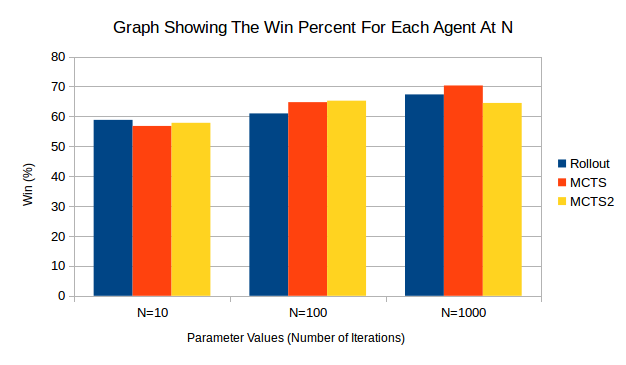
\includegraphics[width=.45\textwidth,scale=.75]{param_comparison_rnd_win}\\
  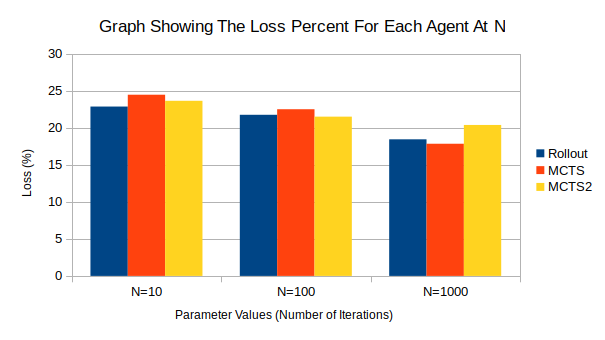
\includegraphics[width=.45\textwidth,scale=.75]{param_comparison_rnd_loss}\\
  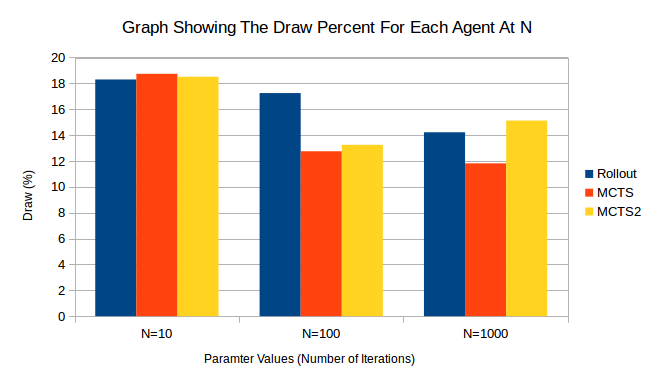
\includegraphics[width=.45\textwidth,scale=.75]{param_comparison_rnd_draw}\\
  % \centering
  \caption{Comparison of Rates of Decision Agents Against An Accumulation Of All The Random Agents Results. Note: A higher the win percent is better but a lower percent is better for the other graphs.}
\end{figure}


\begin{table}[H]
\centering
\caption{Table of Average Decision Times for Decision Agents At Intervals of $N$}
\label{results-table-agent-times}
\def\arraystretch{2.0}%
\begin{tabular}{|l|l|l|l|}
\hline
\textbf{Agent}   & \textbf{N=10 (secs)} & \textbf{N=100 (Secs)} & \textbf{N=1000 (Secs)} \\ \hline
\textbf{Rollout} & 0.111459             & 1.47849               & 108.055421519          \\ \hline
\textbf{MCTS}    & 0.0920657            & 1.52643               & 103.5874541284         \\ \hline
\textbf{MCTS2}   & 0.0894733            & 1.50069               & 92.4551747475          \\ \hline
\end{tabular}
\end{table}

\noindent Note: In table (\ref{results-table-agent-times}) that the MCTS2 is the fastest agent whilst the Random Roll-out is the slowest agent.

\subsection{MCTS Agents}
From the table (\ref{results-table-avr}) the standard MCTS implementation (MCTS) can be seen to work exceptionally well against the random agents. Even at a small number of iterations ($N=10$) it can be seen in the table (\ref{results-table-ai}) that the agent is able to win more than the random agents. It is however evenly matched with the random roll-out agent in this configuration. This is because at 10 iterations the algorithm will barely cover all the possible moves available in a given round (i.e. cards in the players hand) so it will effectively be doing random roll-outs and will not build a very deep tree. As $N$ increases however, MCTS becomes a far better agent than the random roll-outs one. MCTS begins to win considerably more games over roll-out with far fewer draws. At $N=1000$ MCTS is the most successful agent in comparision to all of its opponents as seen in table (\ref{results-table-avr}) and table (\ref{results-table-rnd-results}).  \\

\begin{table}[H]
\centering
\caption{Table of Empirical Results For Decision Making Agents Played Against Each Other (Over 1000 games), $N$ is the number of iterations}
\label{results-table-ai}
\begin{tabular}{|l|l|l|l|l|}
\hline
\textbf{Agents (P1 vs P2)}    & \textbf{N} & \textbf{P1 Wins(\%)} & \textbf{P2 Wins(\%)} & \textbf{Draws(\%)} \\ \hline
\textbf{Heuristic vs Rollout} & 10                      & 33                    & 36                    & 31               \\ \hline
\textbf{Heuristic vs MCTS}    & 10                      & 21                    & 40                    & 39               \\ \hline
\textbf{Heuristic vs MCTS2}   & 10                      & 26                    & 42                    & 32               \\ \hline
\textbf{Heuristic vs Rollout} & 100                     & 34                    & 36                    & 30               \\ \hline
\textbf{Heuristic vs Rollout} & 1000                    & 35                    & 33                    & 32              \\ \hline
\textbf{Heuristic vs MCTS}    & 100                     & 28                    & 54                    & 18               \\ \hline
\textbf{Heuristic vs MCTS}    & 1000                    & 16                    & 63                    & 21               \\ \hline
\textbf{Heuristic vs MCTS2}   & 100                     & 27                    & 54                    & 19               \\ \hline
\textbf{Rollout vs MCTS}      & 10                      & 35                    & 33                    & 32               \\ \hline
\textbf{Rollout vs MCTS2}     & 10                      & 29                    & 39                    & 32               \\ \hline
\textbf{Rollout vs MCTS}      & 100                     & 26                    & 58                    & 16               \\ \hline
\textbf{Rollout vs MCTS}      & 1000                    & 26                    & 51                    & 23               \\ \hline
\textbf{Rollout vs MCTS2}     & 100                     & 16                    & 64                    & 20               \\ \hline
\textbf{MCTS vs MCTS2}        & 10                      & 46                    & 40                    & 14               \\ \hline
\textbf{MCTS vs MCTS2}        & 100                     & 51                    & 39                    & 10               \\ \hline
\end{tabular}
\end{table}

The second MCTS agent (MCTS2) appears to produce very similar results to the original algorithm (In table \ref{results-table-ai}). It is weaker and wins less games than the vanilla algorithm but is much faster (on average decisions) than the vanilla algorithm as seen in figure (\ref{avg-agent-graph}) and table (\ref{results-table-avr}). This is because the search space in the generated tree is greatly reduced. If the loss of accuracy in decision making is acceptable for the increase in decision speed than this algorithm would be a good choice. The random rollout agent does become a better at the game when the number of iterations increases. This is because MCTS2 does not take into account all the possible actions available whereas the random rollout agent (given enough iterations) will consider all actions multiple times.

\begin{figure}[ht]
  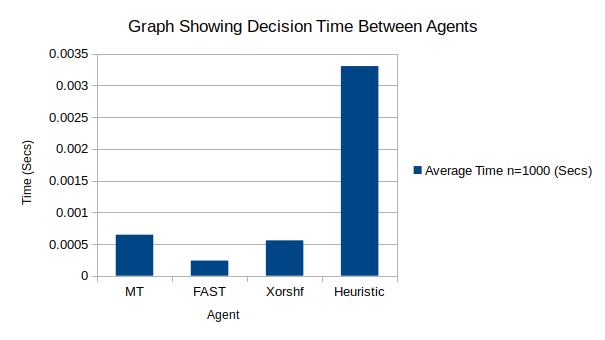
\includegraphics[width=.45\textwidth,scale=.50]{agent_avg_time_s}\\
  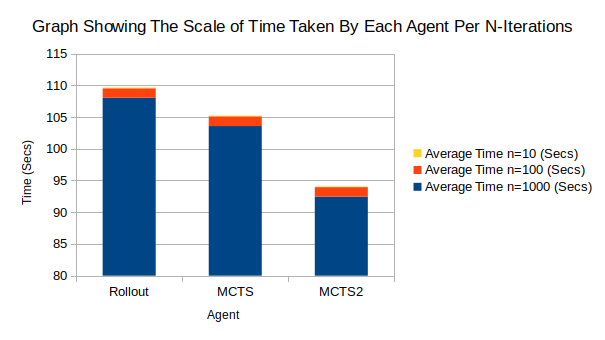
\includegraphics[width=.45\textwidth,scale=.50]{agent_avg_time_n}\\
  \centering
  \caption{Average Decision Time of Agents}
  \label{avg-agent-graph}
\end{figure}

\noindent Note: In figure (\ref{avg-agent-graph}) that the average time for $n=10$ is so small in comparison to the other values for n that it does not register on the graph.

\begin{table}[h]
\centering
\caption{Table of Empirical Results For Decision Making Agents Versus The Random Agents (Over 1000 games, $N$=1000)}
\label{results-table-avr}
\begin{tabular}{|l|l|l|l|}
\hline
\textbf{Agents (P1 vs P2)}      & \textbf{P1 Wins (\%)} & \textbf{P2 Wins (\%)} & \textbf{Draws (\%)} \\ \hline
\textbf{Heuristic vs MT}        & 31.82                 & 34.22                 & 33.96               \\ \hline
\textbf{Heuristic vs Fast Rand} & 99.34                 & 0.48                  & 0.18                \\ \hline
\textbf{Heuristic vs XorShift}  & 31.97                 & 34.67                 & 33.36               \\ \hline
\textbf{Rollout vs MT}          & 51.875                & 28.125                & 20.0                \\ \hline
\textbf{Rollout vs Fast}        & 97.5                  & 0.0                   & 2.5                 \\ \hline
\textbf{Rollout vs XorShift}    & 55                    & 28.125                & 16.875              \\ \hline
\textbf{MCTS vs MT}             & 61.82                 & 25.45                 & 12.72               \\ \hline
\textbf{MCTS vs Fast}           & 99.09                 & 0.0                   & 0.91                \\ \hline
\textbf{MCTS vs XorShift}       & 60.45                 & 25.0                  & 14.55               \\ \hline
\textbf{MCTS2 vs MT}            & 49.5                  & 32                    & 18.5                \\ \hline
\textbf{MCTS2 vs Fast}          & 99.0                  & 0                     & 1.0                 \\ \hline
\textbf{MCTS2 vs XorShift}      & 54                    & 25.0                  & 21.0                \\ \hline
\end{tabular}
\end{table}

\section{Conclusion and Future Research}
These AI agents have shown that the game of Gwent is not solely determined by chance but that strategy also plays a role in the outcome of a game. The Random agents have been beaten by the agents who explore thier action space and the resultant outcomes of those actions. The heuristic AI did not perform as expected which shows that whilst the game is not random, a heuristic which relies on a linear combination of facts from the current game state is too brittle an AI to make informed decisions within the game. The brute force approach of simulating all possible moves in the game has benefits and will produce usable decision but it is a limited strategy which does not work well in very large domains such as Gwent. MCTS helps to solve this problem by limiting its search space in the regions of the state-space where the decisions are promising. This means that MCTS is able to find good decisions often but requires lots of memory and computational time. MCTS is however also used as a base framework for far more complex algorithms which apply other AI and algorithmic techniques to improve the perforamce of such tree search algorithms. MCTS was also shown to be the most successful agent when run against all the other agents that were implemented.\\

Gwent is a complex and interesting domain which has provided a challenge which incorporates stochasticity and non-linear decision making to the problem posed to the AI agents. This project was limited in scope. Future work should look at opening up the domain to more complex rule sets and adding in extra hidden information such as making the opposing decks unknown. Another interesting avenue would be to have the oppenents know each other's hands but not their own hands. The heuristic should also be improved by using more paramters which are trained over random games and the implementation of logic based strategies should also be investigated as a possible heuristic AI. Research into random sampling techniques and machine learning to assist MCTS in sampling good moves is another anvenue of interest.
  
\section*{Acknowledgements}
I would like to acknowledge Dr. Richard Klein for his help and support with debugging the implementation of the testing framework used in this project. I would also like to thank Mr Steven James for his help and support in our discussions about tree search agents and MCTS-based algorithms.\\

Finally I want to state that all intellectual property associated with the game Gwent (such as images of cards) is owned by CD PROJEKT RED and this property has been used according to the Gwent Fan Content Guidelines for an unofficial fan work \cite{cdp}.


% if have a single appendix:
%\appendix[Proof of the Zonklar Equations]
% or
%\appendix  % for no appendix heading
% do not use \section anymore after \appendix, only \section*
% is possibly needed

% use appendices with more than one appendix
% then use \section to start each appendix
% you must declare a \section before using any
% \subsection or using \label (\appendices by itself
% starts a section numbered zero.)
%


% \appendices
% \section{Proof of the First Zonklar Equation}
% Some text for the appendix.

% use section* for acknowledgement
\section*{Glossary of Terms}
\begin{table}[H]
\centering
\begin{tabular}{ll}
\textbf{Abbreviation} & \textbf{Meaning}                          \\
\textbf{AB}           & Alpha-Beta                                \\
\textbf{AI}           & Artificial Intelligence                   \\
\textbf{ACML}         & Adaptive Computation and Machine Learning \\
\textbf{BMCTS}        & Beam Monte-Carlo Tree Search              \\
\textbf{DIP}          & Digital Image Processing                  \\
\textbf{HPC}          & High Performance Computing                \\
\textbf{ISMCTS}       & Information Set Monte-Carlo Tree Search   \\
\textbf{MCS}          & Monte-Carlo Simulation                    \\
\textbf{MCTS}         & Monte-Carlo Tree Search                   \\
\textbf{MCTS-MB}      & MCTS with Minimax Backpropagation         \\
\textbf{MCTS-MR}      & MCTS with Minimax Rollouts                \\
\textbf{MCTS-MS}      & MCTS with Minimax Selection               \\
\textbf{MDP}          & Markov Decision Processes                 \\
\textbf{MT}           & Mersenne Twister                          \\
\textbf{PRNG}         & Pseudo-Random Number Generator            \\
\textbf{UCB}          & Upper Confidence Bounds                   \\
\textbf{UCT}          & Upper Confidence Bounds for Trees         \\
\textbf{XorShft}      & Xorshift                                 
\end{tabular}
\end{table}

% Can use something like this to put references on a page
% by themselves when using endfloat and the captionsoff option.
\ifCLASSOPTIONcaptionsoff
  \newpage
\fi



% trigger a \newpage just before the given reference
% number - used to balance the columns on the last page
% adjust value as needed - may need to be readjusted if
% the document is modified later
%\IEEEtriggeratref{8}
% The "triggered" command can be changed if desired:
%\IEEEtriggercmd{\enlargethispage{-5in}}

% references section

% can use a bibliography generated by BibTeX as a .bbl file
% BibTeX documentation can be easily obtained at:
% http://www.ctan.org/tex-archive/biblio/bibtex/contrib/doc/
% The IEEEtran BibTeX style support page is at:
% http://www.michaelshell.org/tex/ieeetran/bibtex/
%\bibliographystyle{IEEEtran}
% argument is your BibTeX string definitions and bibliography database(s)
%\bibliography{IEEEabrv,../bib/paper}
%
% <OR> manually copy in the resultant .bbl file
% set second argument of \begin to the number of references
% (used to reserve space for the reference number labels box)
% \begin{thebibliography}{1}

% \bibitem{AIModern}
% Russell, Stuart and Norvig, Peter, \emph{{Artificial Intelligence: A Modern Approach}}, 3rd~ed.\hskip 1em plus
%   0.5em minus 0.4em\relax Pearson, 2009.
  
% \bibitem{mitchell}
% Mitchell, T.M. \emph{{Machine Learning}}, \hskip 1em plus
%   0.5em minus 0.4em\relax McGraw-Hill, 1997. 


% \end{thebibliography}

\bibliographystyle{plain}
\bibliography{biblist}{}

% biography section
% 
% If you have an EPS/PDF photo (graphicx package needed) extra braces are
% needed around the contents of the optional argument to biography to prevent
% the LaTeX parser from getting confused when it sees the complicated
% \includegraphics command within an optional argument. (You could create
% your own custom macro containing the \includegraphics command to make things
% simpler here.)
%\begin{biography}[{\includegraphics[width=1in,height=1.25in,clip,keepaspectratio]{mshell}}]{Michael Shell}
% or if you just want to reserve a space for a photo:

% \begin{IEEEbiography}[{\includegraphics[width=1in,height=1.25in,clip,keepaspectratio]{picture}}]{John Doe}
% \blindtext
% \end{IEEEbiography}

% You can push biographies down or up by placing
% a \vfill before or after them. The appropriate
% use of \vfill depends on what kind of text is
% on the last page and whether or not the columns
% are being equalized.

%\vfill

% Can be used to pull up biographies so that the bottom of the last one
% is flush with the other column.
%\enlargethispage{-5in}



% that's all folks
\end{document}


